\documentclass{UoNMCHA}
\usepackage[authoryear]{natbib}
\usepackage{array,booktabs} % For nice tables
\usepackage{amsmath,amsfonts,amssymb} % For nice maths
\usepackage{color}
\usepackage{enumerate}
\usepackage{listings}
\usepackage{subfig}
\usepackage{hyperref}
\usepackage{pdfpages}
\usepackage[parfill]{parskip}   % For replacing paragraph indenting with a newline instead

% Number equations per section
\numberwithin{equation}{section}

\hypersetup{
%    bookmarks=true,         % show bookmarks bar?
%    unicode=false,          % non-Latin characters in AcrobatÕs bookmarks
%    pdftoolbar=true,        % show AcrobatÕs toolbar?
%    pdfmenubar=true,        % show AcrobatÕs menu?
%    pdffitwindow=false,     % window fit to page when opened
%    pdfstartview={FitH},    % fits the width of the page to the window
%    pdftitle={My title},    % title
%    pdfauthor={Author},     % author
%    pdfsubject={Subject},   % subject of the document
%    pdfcreator={Creator},   % creator of the document
%    pdfproducer={Producer}, % producer of the document
%    pdfkeywords={keyword1} {key2} {key3}, % list of keywords
%    pdfnewwindow=true,      % links in new window
    colorlinks=true,       % false: boxed links; true: colored links
    linkcolor=blue,          % color of internal links
    citecolor=blue,        % color of links to bibliography
%    filecolor=magenta,      % color of file links
    urlcolor=blue           % color of external links
}

\definecolor{MATLABKeyword}{rgb}{0,0,1}
\definecolor{MATLABComment}{rgb}{0.1328125,0.54296875,0.1328125}
\definecolor{MATLABString}{rgb}{0.625,0.125,0.9375}

\lstset{language=Matlab,
    basicstyle=\small\ttfamily,
    keywordstyle=\color{MATLABKeyword},
    %identifierstyle=,
    commentstyle=\color{MATLABComment},
    stringstyle=\color{MATLABString},
    numberstyle=\tiny,
    %numbers=left,
    basewidth=0.5em}

\firstpage{1}    % Set page number for first page
\UoNMCHAreportNo{MECH4841 Part B} %Report number
\UoNMCHAyear{2013}   % Year
\shorttitle{FYP Report - Optical Flow Based Obstacle Avoidance} %For odd pages
%%%%%%%%%%%%%%%%%%%%%%%%%%%%%%%
\begin{document}

\includepdf[pages=-]{FYP_Cover_Page.pdf} % //TODO: Includes Coversheet PDF, Needs to be Filled out
\title{Optical Flow Based Obstacle Avoidance for a Fixed Wing UAV\\ \ \\
{\small Final Year Project Report - MECH4841 Part B  \\June 2019}}
\author[UoNMCHA]{Patrick Prell}
\address[UoNMCHA]{
Student of Mechatronics Engineering,\\
The University of Newcastle, Callaghan, NSW 2308, AUSTRALIA \\
Student Number: 3204734 \\
E-mail: \href{mailto:Patrick.Prell@uon.edu.au}{\textsf{Patrick.Prell@uon.edu.au}}}
%%%%%%%%%%%%%%%%%%%%%%%%%%%%%%%
\maketitle
\onecolumn

\vspace{-5mm}
\section*{Abstract}
\vspace{-3mm}
Remember that executive summary may include the following information:
\begin{itemize}
    \item Defines the intention of the report.
    \item Places the report in context so the reader knows why it is important to read it.
    \item Why is it important?
    \item What problem is addressed?
    \item Briefly states the results
    \item Briefly presents the implications and recommendations
\end{itemize}
%%%%%%%%%%%%%%%%%%%%%%%%%%%%%%%
\vspace{-2mm}
\section*{Acknowledgements}
\vspace{-3mm}
You may like to say thank you to someone that helped you with your project.
%%%%%%%%%%%%%%%%%%%%%%%%%%%%%%%
\newpage
\tableofcontents
\newpage
%%%%%%%%%%%%%%%%%%%%%%%%%%%%%%%
\section{Introduction}
To organise your introduction section you can use the following structure:
\begin{itemize}
    \item \textbf{Position}: Show there is a problem and that it is important to solve it.
    \item \textbf{Problem}: Describe the specifics of the problem you are trying to address
    \item \textbf{Proposal}: Discuss how you are going to address this problem. Use the literature to back-up your approach to the problem, or to highlight that what you are doing has not been done before
\end{itemize}

The rest of the report is organised as follows. Section~\ref{sec:Background} describes items related to the core content. Section~\ref{sec:Conclusion} concludes the report. Appendix~\ref{app:Table} shows an example of how to make a Table.

%%%%%%%%%%%%%%%%%%%%%%%%%%%%%%%
\section{Background}\label{sec:Background} %FIX THIS!!!
To the average human or most mammals for that matter, visual tasks such as identifying objects and interpreting visual cues come as second nature. However, implementing algorithms that mimic this ability is infuriatingly difficult. What is often forgotten is that for all of its amazing abilities approximately 1/3 of the human brain is dedicated to analysing the information collected from our eyes. This statistic helps to put into perspective how challenging the field of computer vision can be.

The concept of computer vision has been explored since the beginning of artificial intelligence research in the late 1960’s, with the goal of extracting the 3-Dimensional structure of a scene from images. The following decade saw research attempting to extract more information from a sequence of images using visual cues from the motion of a camera. This brought about work on visual navigation as a viable method to navigate an environment. Using Visual Navigation on a robot to move through an unstructured environment with no prior knowledge of the map is often based on optic flow (Altshuler and Srinivasan, 2018), where a motion field is estimated from fusing the motion of the robot with the motion of the pixels of a video feed. Furthermore, biologically inspired visual navigation techniques have been a topic for research. By observing the way that animals and insects utilise their visual systems to move about and map their environments, the processes for which this is achieved can be replicated and used on a robotic system for similar tasks. This section outlines the planar and spherical model of optic flow, the tools used to infer motion between frames, and how honeybees use Visual Navigation (Srinivasan, 2011).
\subsection{Biological Inspiration} % 1 page
\subsubsection{Visual Navigation}
\subsubsection{}
\subsubsection{}
\subsection{Optic Flow} % 2 pages
The first use
\subsubsection{Horn \& Schunk}
\subsubsection{Lucas - Kanade}
\subsubsection{What is Observable in Optic Flow}
Pose rate estimation

\begin{itemize}
	\item Angular velocity,
	\item reflect on the work presented, 
	\item make recommendations,
	\item suggest future work or improvements.
\end{itemize}

\newpage
\subsection{Camera Calibration}
Computer vision begins with the camera detecting light from a scene. This light has travelled from its source, reflecting from an object, through the camera lens and is recorded on the image sensor. For these rays of light that make up an image to be useful for representing the real-world, we must understand the geometry that transforms these rays from the three-dimensional real world to a two-dimensional image plane i.e. world coordinates to image coordinates.

The camera calibration process describes the camera with two sets of parameters, namely the intrinsic parameters, and the extrinsic parameters. The intrinsic parameters describe the geometric relationship between the camera model and its projection. And the extrinsic parameters describe the location and orientation or pose, of the camera with respect to the world frame.

This project uses a GoPro Hero 7 to test and verify the calibration routine. This section will cover camera models and outline why a planar model is used for the GoPro. It covers the mathematical tools used to capture the different effects that make our camera imperfect for representing the real world, and how we can correct for these deviations.
\subsubsection{Camera Models}
The most elementry way of representing a camera is with the pinhole model. Light enters the appeture (pinhole) after reflecting from objects in a scene. For an ideal pinhole camera, only one ray enters the apeture from any point in the scene. The light is then projected onto a surface behind the appeture resulting in an image of the scene that is scaled proportional to the focal length $f$.

\begin{figure}[ht]
    \begin{center}
        \includegraphics[width=.8\linewidth]{Figures/Pinhole_model}
        \caption{Elementary pinhole model of a camera: In practice, the appeture must be big enough to let light in, allowing a narrow ray of light from each point in the scene blurring the image. Therefore there is a tradeoff between brightness and sharpness.}
        \label{fig:PinholeModel}
    \end{center}
\end{figure}

Figure~\ref{fig:PinholeModel} shows an ideal pinhole camera model and its parameters, where $f$ is the focal length, $Z$ is the distance along the optical axis to an object, $x$ is the size of the projected object and $X$ is the size of the object. For this model, \eqref{eq:pinholeEQ} is the relationship between the projected image and the object
\begin{equation}\label{eq:pinholeEQ}
	\frac{-x}{f} = \frac{X}{Z}
\end{equation}
Due to how light enters the camera, the image of a pinhole model is represented upside down. This issue is fixed in a plainar camera model. The plainar model is similar to a pinhole model, however rather than passing through an appeture, light travels from each point in the scene, intersects the image plane and converges to a single point known as the \textit{Centre of projection}. this concept is best described in Figure~\ref{fig:PlainarModel}, where

\begin{figure}[ht]
    \begin{center}
        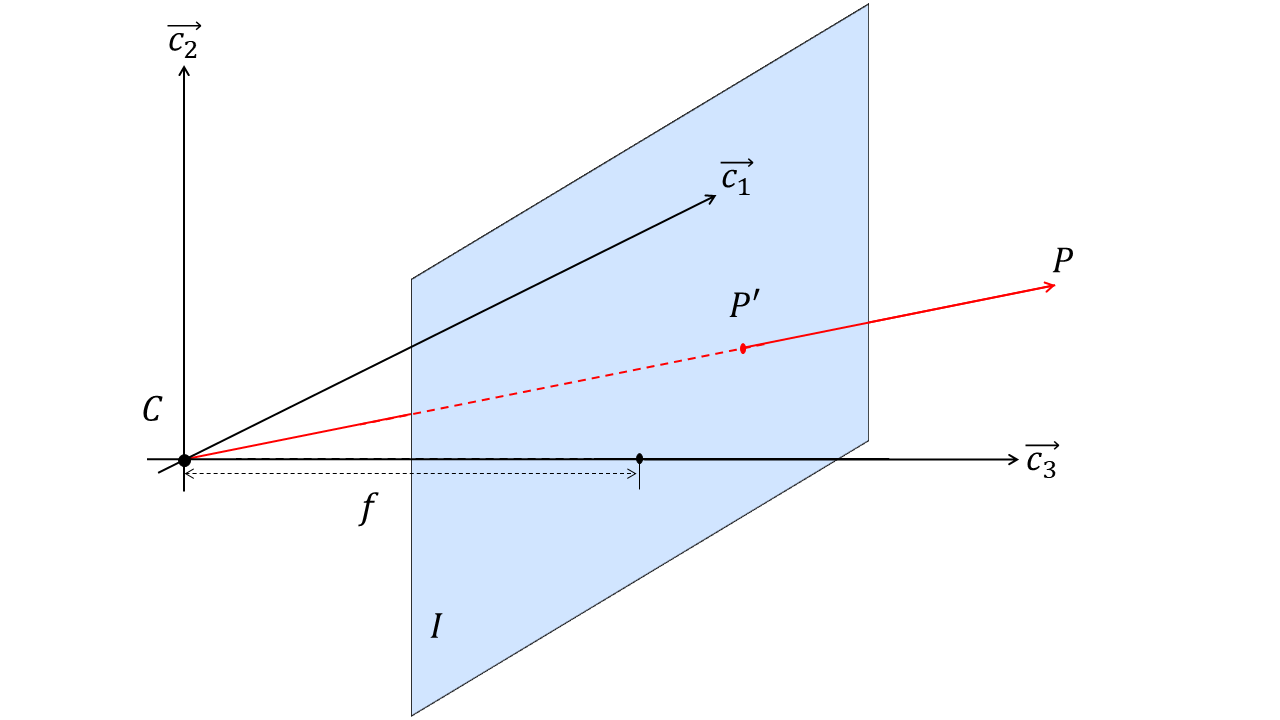
\includegraphics[width=.6\linewidth]{Figures/Planar_Model}
        \caption{}
        \label{fig:PlainarModel}
    \end{center}
\end{figure}

\subsubsection{Projective Transform}
\subsubsection{Homogenius Coordinates}
\subsubsection{Rodrigus Transform}

\subsection{Inverse Optimal Control} % 3 pages
\subsubsection{Sudo Control Algorithm for Insects}
\subsubsection{}
\subsection{Approach}
\subsubsection{Inverse Depth Calculation}
\subsubsection{Unity Simulation}
\subsubsection{Assumptions}
Static environment
using GoPro
Simple aircraft kinematic model
\subsubsection{Simulations}
Kinematic data collected
Used ray cast to gather depth information
\subsubsection{Real World Data}
The project is primaritly simmulation based. However, the camera calibration routine (explored in following sections was tested and evaluated on real world images collected from a GoPro Hero 7. Were this project to be implemented on a real world fixed wing UAV, the kinematic data would need to be obtained through sensors on the UAV. Additionally, the control algorithm
U-Blox RTK GPS module
High Performance MEMS IMU (i.e. )
GoPro Hero
%%%%%%%%%%%%%%%%%%%%%%%%%%%%%%%
\newpage
\section{Optical Flow}
\subsection{Algorithms}
\subsection{Measurement Model}
\subsection{Simulation}
\subsection{Farnback Algorithm - OpenCV}

%%%%%%%%%%%%%%%%%%%%%%%%%%%%%%%
\newpage
\section{Camera Calibration}

%%%%%%%%%%%%%%%%%%%%%%%%%%%%%%%
\newpage
\section{Vector Field Divergence for Object Avoidance}

%%%%%%%%%%%%%%%%%%%%%%%%%%%%%%%
\newpage
\section{Flow Magnatude for Object Avoidance}

%%%%%%%%%%%%%%%%%%%%%%%%%%%%%%%
\newpage
\section{Discussion}

%%%%%%%%%%%%%%%%%%%%%%%%%%%%%%%
\newpage
\section{Conclusion}\label{sec:Conclusion}

%%%%%%%%%%%%%%%%%%%%%%%%%%%%%%%
\newpage
\section{Recomendations}

%%%%%%%%%%%%%%%%%%%%%%%%%%%%%%%
\newpage
\bibliographystyle{harvard}
\bibliography{main} % This is the .bib file where the bibliography database is stored

%%%%%%%%%%%%%%%%%%%%%%%%%%%%%%%
\appendix
\newpage
\section{Journal}\label{app:Journal}

\end{document}